\chapter{Related Work}
\label{cha:Related Work}


The development of self-driving cars represents one of the most intricate and ambitious challenges in the field of engineering, robotics and artificial intelligence. The complexity and variability of real-world driving environments make this task extremely difficult. The environments include unpredictable actors, such as other drivers, pedestrians, and animals, as well as changing weather and road conditions. The environments include uncounted edge cases that are difficult to anticipate and code for explicitly. Consequently, many researchers and institutions include advanced machine learning techniques in their approaches towards solving autonomous driving.

The development of autonomous driving systems started with driver assistance systems in the 1970s. These systems focus on assisting the driver in specific tasks, such as lane keeping, adaptive cruise control, and parking. This reduces the problem complexity. However modern self-driving systems aim to achieve full autonomy. For example the Tesla autopilot is capable of driving in many environments without human intervention.

This thesis will use reinforcement learning in the training of an autonomous driving agent. The agent is equiped with a single camera sensor. The agent's behaviour is controlled by a convolutional neural network that processes the visual input. The agent has to learn a specific self driving task with reduced complexity. The self-driving task is similar to previous research at the ScaDS.AI \textcite{maximilian}. However the agent design and training is very different.
The task consists of a restricted environment. The environment consists of an enclosed arena with different tracks that the agent has to complete. The tracks consist of a series of goals that the agent has to drive through. The tracks are grouped in three difficulty levels.
The environment is simulated with three light settings. The trained agent has to learn to navigate all difficulty levels and light settings.

Research relating to reinforcement learning algorithms, convolutional neural networks and self-driving will be reviewed.
% also research regarding rebustness to light changes?

% TODO auch die Ergebnisse der Paper und die daraus gezogenenn Schlüsselideen erwähnen


\section{Self-Driving}

Neural networks have been used in the domain of self driving for a long time. Pomerleau \textcite{alvinn} developed one for the first self driving systems with neural networks in 1989. The system was developed for road following. The system used a camera image and a laser range finder as input. Compared to current network sizes, they used a small fully connected neural network. The network was trained using synthetic data. The data consisted of generated road images and steering commands. The network was trained using backpropagation to reproduce the steering commands. This approach did not use reinforcement learning. The system was able to follow roads in real-life under certain conditions.
The paper highlights the advantages of neural networks for self-driving. The training data determines the salient image features and not the programmer. This has proven to be true with the success of convolutional neural networks in the domain of self-driving \textcite{neptune}.


There has been a lot of progress in the domain of self-driving in recent years. Sophisticated self-driving algorithms consist of many hardware and software components to achieve satisfying performance. Hardware components include various imaging approches such as Radar, Lidar and cameras. Termometers and other hardware components are also used, for example to determine weather conditions. 
Software components might include separate object detection, occupancy and planning. For example Tesla's self-driving builds these components on top of a shared backbone that uses convolutional neural networks \textcite{howteslaautopilot}.
% (CNN is ResNet)

Self-driving in a real world environment is a very complex task, especially when including other traffic participants. Modern self driving agents consist of multiple complex components that interact with each other \textcite{drl_for_ad}. Components for Scene Understanding build a model of the current surroundings. The Descision making \& Planning components use this model to decide and execute the next actions.
Multiple interacting components are shown in figure \ref{fig:ad_components}.

\begin{figure}
    \centering
    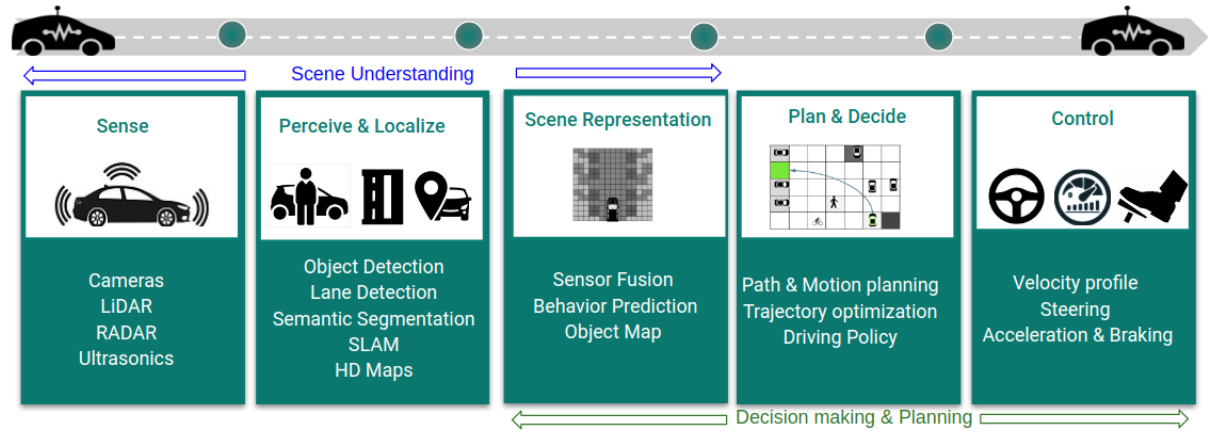
\includegraphics[width=0.8\textwidth]{Bilder/ad_components_from_paper_drl_for_ad.png}
    \caption{Standard components in a modern autonomous driving systems pipeline listing the various tasks. The key problems addressed by these modules are Scene Understanding, Decision and Planning. Image from \textcite{drl_for_ad}}
    \label{fig:ad_components}
\end{figure}

An agent with similarly complex components is not feasible for this thesis. The agent in this thesis uses a single convolutional neural network to process the visual input and make decisions instead. I aim to contribute to the domain by expanding on previous research and focus on the training of a convolutional neural network agent. 


TODO wohin diesen satz?
Approaches from the domain of self-driving will be used to improve the training of the agent, for example reward shaping \textcite{drl_for_ad}.

\subsection{Previous Work}
This thesis builds directly upon the work of Knig \textcite{jonas_koenig}, Flach \textcite{merlin_flach} and Schaller \textcite{maximilian}. 
\textcite{jonas_koenig} built a self-driving agent that was trained to avoid collisions in a simulated arena. The agent used a hand-crafted preprocessing pipeline to extract features from visual input. The features represent the obstacles that the agent has to avoid. The agent's behaviour was controlled by a policy that consisted of a neural network. This network used the extracted features as inputs. It was trained using an evolutionary approach in simulation.

\textcite{merlin_flach} investigated the feasibility of transferring this agent to the real world. The research showcased many challenges. The challenges are caused by differences between the simulated and real-life environments, the Simulation-To-Reality gap. The most notable problem was the object recognition part. The preprocessing pipeline had difficulties recognizing the objects in the real world. This results in further problems for the agent, since the agent's policy is based on the extracted features.

\textcite{maximilian} investigated a different task than the two previous papers. An agent was trained to traverse a track by driving through a sequence of goals. The same tracks are used in this paper. The agent used a preprocessing pipeline to extract object features similar to \textcite{jonas_koenig}. The neural network policy was trained using the proximal policy optimization \textcite{ppo} reinforcement learning algorithm. The agent could traverse the tracks, its performance decreased for tracks of higher difficulty. Further evaluation of the agent under different light settings showed that the agent is not robust to changing light conditions. The preprocessing pipeline was not able to extract the necessary features reliably under different light settings, this resulted in a performance collapse.

The instability of the hand-crafted preprocessing pipeline and promissing results by CNNs from other RL researchers in the domain of self-driving \textcite{neptune} motivate the choice of CNNs as the feature extraction method in this thesis. 


\section{Reinforcement Learning}

% data not programmer decides the salient image pixels (bedeutungsvollen)
\subsection{Introduction to Reinforcement Learning}

Reinforcement Learning algorithms have been around for a long time, but only recently have they been able to achieve superhuman performance in games and control tasks \textcite{atari}. Reinforcement learning algorithms formalize the problem as consisting of an environment and a policy $\pi$. The environment consists of a state space, an action space and a reward function that takes state-action pairs as input. Reward functions assign positive rewards to actions that are deemed to be desirable by the environment designers, for example scoring a goal in a football match. Reward function can also assign negative rewards to undesirable actions, for example collisions in a driving simulation. 

The goal of reinforcement learning algorithms is to build an agent that interacts with its environment and maximizes the cumulative reward over time. The policy selects actions given an observation. It controls the agents behaviour \textcite{rlbook2020}. It is trained by the \acs{RL} algorithm to learn the desired behaviour. The trained policy can then be used to solve problems in the environment. 

The agent interacts with the environment during the training phase of RL algorithms. The policy takes some representation of the environment's state as input and selects actions to execute in the environment. The selected actions are executed in the environment by the agent which results in a new state. The reward function assigns rewards to these state transitions.
The observed rewards are then used to update the policy \ref{fig:rlcycle}.

\begin{figure}
    \centering
    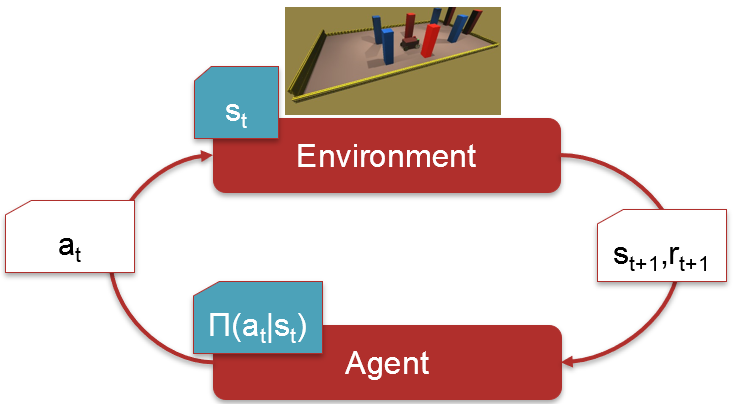
\includegraphics[width=0.4\textwidth]{Bilder/rl_cycle.png}
    \caption{RL Training Cycle: The agent selects action $a_t$ based on policy $\pi(a_t|s_t)$ at state $s_t$ and recieves the next state $s_{t+1}$ and rewards $r_{t+1}$ from the environment. The states, actions and observed rewards are used to update the policy.}
    \label{fig:rlcycle}
\end{figure}

\subsection{Classification of \acs{RL} Algorithms}

Reinforcement learning algorithms are classified into two major groups. RL algorithms that use a model of the environment are called model-based algorithms, algorithms without such models are called model-free algorithms. Algorithms from both groups have been successfully used in a wide range of applications, model-based algorithms are often much more complex but have been shown to be successful at many task that require planning \textcite{alphagoimprovementmuzero}. Model-free approaches are often simpler and more flexible, they have shown great success in various control tasks \textcite{atari}.

\begin{figure}
    \centering
    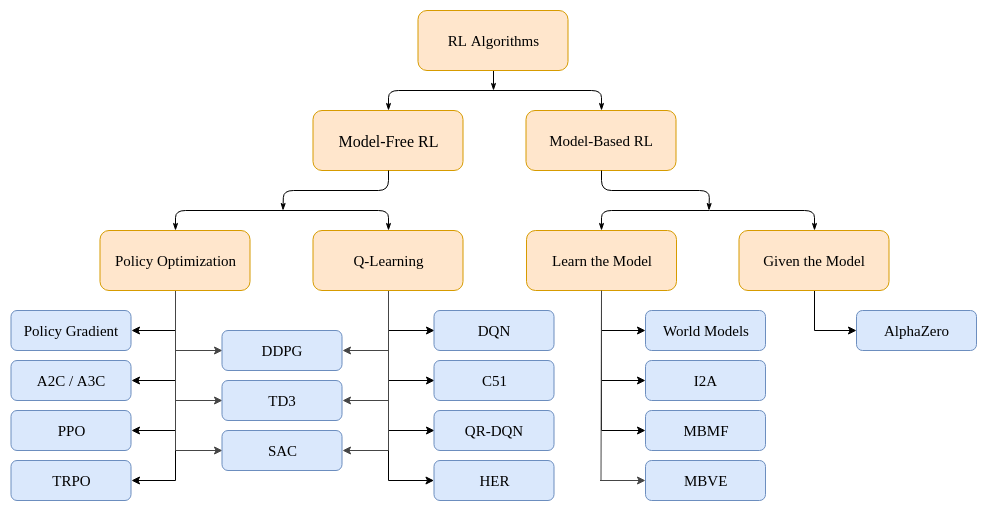
\includegraphics[width=0.8\textwidth]{Bilder/openai_spinningup_taxonomy.png}
    \caption{Taxonomy of RL algorithms from OpenAI's Spinning Up course \autocite{spinningup}}
\end{figure}

\subsubsection{Model free \acs{RL} Algorithms}

\paragraph{Value based algorithms}
Model free algorithms can be further divided into two families. The first family are value-based approaches. These algorithms learn a function that assigns state-action pairs a value. This function is called the value function. This value represents the expected future reward Q.
 
The policy is not trained directly. The policy selects actions based on this value function instead. The state-action pair with the highest Q-value is selected for a given state.

The training process of the value function is done by updating the Q-values based on the observed rewards. The Q-learning algorithm is an early and common example of value-based algorithms \textcite{rlbook2020}. The Q-learning algorithm updates the values based on the observed rewards and the maximum Q-value of the next state \[Q(S_t, A_t) = Q(S_t, A_t) + \alpha (R_{t+1} + \gamma \max_a Q(S_{t+1}, a) - Q(S_t, A_t))\].
$\alpha$ is the learning rate. It determines how quick values are changed. $\gamma$ is the discount factor of future rewards.


The Q-learning algorithm can use a table to store the value function. The table contains one cell for each state-action pair and stores the Q-value. 
For many problems the use of these tables in not feasible due to the amount of state-action pairs, many extensions to the algorithms have been developed such as for example deep q-learning. Deep q-learning uses a deep neural network to approximate the Q-values \textcite{atari}. The network learns to predict the Q-values for state-action pairs. Neural networks are general approximators. They can learn to generalize and return accurate value predictions even for previously unseen states.  

Value-based \acs{RL} algorithms have been used to great success for control tasks \textcite{rlbook2020}. However they will not be used in this thesis, as they require discrete action spaces. The environment in this thesis consists of a continuous action space.
An action space can be discretized for use by value-based algorithms \ref{fig:example_discretization}. However this can lead to a loss of fidelity.

% TODO \ref{fig:example_discretization} ?

\paragraph{Policy based algorithms}
% rlbook2020 chapter 13.7
The other family are policy-based algorithms. These algorithms optimize the policy directly instead of the values associated with states or state-action pairs. Instead of computing the learned probability of each action, the policy learns the statistics of the action distribution.
Given a scalar action space. The action distribution can be represented as a gaussian probability Distribution:
\[p(x) = \frac{1}{\sqrt{2\pi\sigma^2}} e^{-\frac{(x-\mu)^2}{2\sigma^2}}\]

The policy can then be defined as the normal probability density over a real-valued scalar action. The mean and standard deviation of the distribution are given by parametric function approximators that depend on the state $s$. The mean is given by $\mu(s, \theta)$ and the standard deviation by $\sigma(s, \theta)$. The policy is then defined as:
\[\pi(a|s, \theta) = \frac{1}{\sigma(s, \theta)\sqrt{2\pi}} e^{-\frac{(a-\mu(s, \theta))^2}{2\sigma(s,\theta)^2}}\]

The parametric function approximators $\mu(s, \theta)$ and $\sigma(s, \theta)$ are trained by the \acs{RL} algorithm. Any function approximator can be used, for example a \acs{NN} with parameters $\mu$ \textcite{rlbook2020}. 

The action distribution can be extended to multi-dimensional action spaces. This action distribution can be represented as a multivariate gaussian distribution. The function approximator then outputs the mean and covariance matrix of the distribution. This makes policy-based \acs{RL} algorithms very flexible. They can be used for multi-dimensional continuous action spaces.


The policy can be updated using the gradient of the expected rewards with respect to the policy parameters. Algorithms that use this approach are called policy gradient algorithms.


\paragraph{Actor-Critic Algorithms}
Alternatively the policy can be updated using Actor-Critic approaches. These combine policy-based and value-based approaches. Actor-Critic approaches contain a policy and a value function. The value function represents the expected future reward of a state. The policy is updated using this value function.

The Proximal Policy Optimization algorithm is an Actor-Critic algorithm. It was developed to improve the stability of policy-based algorithms \textcite{ppo}. The \acs{PPO} algorithm restricts the size of policy changes caused by parameter updates, which ensures the policy does not change drastically. This improves stability. \acs{PPO} is currently one of the most popular algorithms for reinforcement learning. It has already been successfully used in the domain of autonomous driving \textcite{maximilian}.



% Another major improvement in the domain of reinforcement learning was the combination of neural networks with traditional planning and search algorithms, the most famous example for this is AlphaGo \textcite{alphago}. These algorithms often are model-based algorithms and use search algorithms (e.g. Monte Carlo Tree Search)  to evaluate the possible actions at a given state. The neural networks are used for the evaluation of states and actions in the search algorithms. AlphaGo was developed for a 2 player deterministic game with a discrete state and action space. Since then this combination of neural networks and search algorithms has also been used to achieve impressive results for all kinds of problems \textcite{alphafold}, for example single player continuous state and action spaces \textcite{alphagoimprovementmuzero}. Although these algorithms could be applied to the problem at hand, they will not be utilized due to the increased complexity of the algorithms and the required computational resources.
% TODO sollte der Teil wieder rein?

% temporal difference learnign: update a function based on previously learned things (e.g. q-learning)

% TODO mention reward shaping from rlbook somewhere
% first give a reward signal that is not aligned with final goal but gives frequent rewards
% train the agent using this function
% change function over time to the intended reward function (event Reward)
% learning behaviour is guided by the shaped reward function



\subsection*{Convolutional Neural Network for Reinforcement Learning}

Convolutional neural networks are a neural network architecture specifically developed for processing image data, they consist of a number of filters and a fully connected neural network. The filters are applied to the image in a sliding window fashion, the filters detect patterns in the image such as for example edges and corners. Multiple successive applications of such filters enables the network to learn hierarchical information and recognize more complex structures. The fully connected neural network analyses the results of the filters and makes the final prediction \textcite{rlbook2020}.

CNNs are often used in Reinforcement Learning since RL problems often require an agent to process visual input. Furthermore CNNs can be trained end-to-end in Reinforcement Learning compared to other feature extraction methods, which means the CNN can learn what features are important for the task at hand.
Therefore a convolutional neural network will be used to process the camera images instead of a hand-crafted feature extraction method. 

CNNs typically do not take the raw camera/simulation images but rather preprocessed images, e.g. greyscaled images \textcite{atari}. Preprocessing steps can help in reducing the complexity of the input space. Convolutional neural networks require a lot of data to train, data augmentation can help increase the size of the training set and to make the agent more robust. Data augmentation generates new samples from already collected ones by applying transformations to the samples. 


% TODO move next paragraph to CNN section?
The PPO algorithm can be used to train agents that use convolutional neural networks as their policy. Convolutional neural networks are ideal for processing image data and can be trained end-to-end by the algorithm \textcite{ppo}. 

% rlbook2020 chapter 9.7 explains the use of CNNs in RL



% \textcite{autonomous_vehicles_review} %TODO read this paper and cite it

% https://safe-intelligence.fraunhofer.de/en/autonomous-driving

% Papers that use Carla



\section{Simulation for Reinforcement Learning and Self-Driving}

% TODO Carla und andere Simulations machen keinen Sinn, da wir ein festse Problem haben

Simulations play a huge role in reinforcement learning and thus the development of self-driving agents. Simulations provide a huge number of benefits over real world experiments. They are much cheaper and faster to run than real world experiments, furthermore they can be run in parallel. In addition the programmers have direct and perfect control over the environment, as such programmers can for example change the simulation speed. This allows for fast experimentation and training of reinforcement learning agents. Simulations also allow for the creation of scenarios that are not possible in the real world. This is especially useful for reinforcement learning agents that are trained to avoid collisions. Simulations also allow for the creation of ground truths such as perfect sensor data and object bounding boxes \textcite{carla}.

Simulated environments often serve as baselines for reinforcement learning algorithms, most famous are the atari games \textcite{atari}. The Python Gynasium API was developed for easy reuse and comparison of reinforcement learning algorithms for different problems \textcite{gymnasium}, the Gymnasium API defines an interface that can be used to model tasks as reinforcement learning problems. A wide range of reinforcement learning frameworks support the Gymnasium API, for example Google's dopamine \textcite{dopamine} and OpenAI's baselines \textcite{sb3}. Advanced simulations like the Unity engine \textcite{unity}, the physics simulator MuJoCo \textcite{mujoco} and the driving simulator Carla \textcite{carla} can be integrated with the Gymnasium API.

%The complexity and interest in self-driving has also led to the development of dedicated simulators, such as the Carla \textcite{carla} and the AirSim \textcite{airsim} simulator. The Carla simulator provides researchers with useful features such as weather control and ground truths for object detection and segmentation.

There are also dedicated frameworks for reinforcement learning that directly integrate with simulation engines. \textcite{maximilian} used the ML-Agents framework \textcite{mlagents} to train the self-driving agent in Unity directly.

In this thesis Unity will be used for the simulation, the simulation will be integrated with the Python Gymnasium API and PPO algorithm. This approach is chosen instead of the ML-Agents framework since it allows for more flexibility and control over the simulation and training process.


\section{Imitation learning}
As described before it is difficult to build self-driving agents for real world environments due to the environment complexity. The amount of complex edge cases make it very difficult to programmatically define the agent's behaviour. Neural networks can be used to control the agent behaviour instead. The neural networks can be trained using reinforcement learning in simulation. 
Imitation learning is another approach to training an agent that interacts with its environment. Imitation learning requires a dataset that demonstrates the desired behaviour. The agent is trained on the dataset to mimic the expert behaviour.

In reinforcement learning the programmer has to define a reward function that the agent uses to learn and improve its behaviour. In imitation learning the agent learns exclusively from the dataset. As a result this dataset has to include a wide range of scenarios to produce a reliable agent that can handle edge cases.

There are two approaches to training an agent with imitation learning, behavioural cloning and inverse reinforcement learning. Behavioural cloning is the simpler approach, the agent learns to mimic the expert behaviour directly. This is similar to supervised learning. Inverse reinforcement learning is more complex, the reward function from the expert demonstrations is learned first. The agent is then trained to maximize this reward function using reinforcement learning. 

Bojarski \textcite{bojarski2016endToEnd} used imitation learning to train a self-driving lane following agent for real-world environments. This agent consists of a convolutional neural network that processes the camera images and predicts the steering angle directly. The agent is trained end-to-end to reproduce steering behaviour from recorded data. They demonstrate that imitation learning is a viable approach for developing an agent without the need for multiple components such as object detection and path planning.

Tesla used imitation learning to train the path prediction component of their self-driving systems. The fleet of Tesla vehicles allows them to collect a large amount of representative data in the real world. The reference dataset was generated from recordings of human Tesla drivers \textcite{tesla_youtube}. 

Imitation learning and reinforcement learning can be combined to improve the training of the agent. The reinforcement learning process generates samples via interaction between agent and environment. These samples and the expert behaviour dataset are used together to train the agent policy \textcite{car-following_carla_dresden}.


%\section{Reinforcement Learning for Self-Driving}

%\textcite{drl_for_ad} review the use of reinforcement learning for autonomous driving, they also describe many improvements for reinforcement learning algorithms that can improve the training stability and performance, such as for example reward shaping.
%In addition to published research papers there have been a lot of experiments, tutorials and demonstrations of self-driving agents on YouTube and GitHub. The University of Tübingen published their full lecture series on Self-Driving Cars \textcite{tuebingen}, the series also includes a section on reinforcement learning.

% papers that cite carla: https://scholar.google.de/scholar?cites=660591080772510291&as_sdt=2005&sciodt=0,5&hl=de


% Tübingen: % https://www.youtube.com/watch?v=GYnlqiSqZiU&list=PL05umP7R6ij321zzKXK6XCQXAaaYjQbzr&index=13



% Key Papers in RL: https://spinningup.openai.com

\section{Light change resiliency}

\subsection{Domain Randomization}

useful for transfer sim-to-real
https://ar5iv.labs.arxiv.org/html/1703.06907

domain randomization for sim-to-real tries to teach the agent to solve a task under a big variety of conditions in simulation, the hope is that the agent will be able to generalize this variation and learn in this environment.
The real world is simply one variety that the agent might have already learned to generalize.

The randomization can include textures, image resolutions, ..., motor power of agent in sim, ... (physical properties)


domain randomization can lead to a high variance of policy performance for different environment randomizations. The paper https://ar5iv.labs.arxiv.org/html/1910.10537 introduces a regularization approach for the policies.
visual vs dynamics randomization (camera changes vs physics e.g. friction of wheels)

\subsection{Data augmentation}

Data is collected in simulation and then augmented


\subsection{Multi-Modal learning}

Provide the agent with more than just image data,  e.g. radar...


\subsection{Hierarchical Reinforcement Learning}

combination of multiple levels. higher level policy controlls the actions, the lower level policy learns to build representations for the higher level policy

Hierarchical Reinforcement Learning: Using a hierarchical approach where high-level policies govern low-level policies can help the agent adapt to changing conditions more effectively. High-level policies can decide on strategies based on the overall environment, while low-level policies handle specific tasks like adjusting to lighting changes


TODO relate the previous work that used a hand-crafted feature extraction pipeline to hierarchical rl

\section{Transfer to reality}

\subsection{Transfer Learning}
learn on diverse data and then fine-tune on real data


\section{Key Ideas}

\subsection{Fitting RL algorithms}

\subsubsection{CNN for feature extraction in RL}

\subsubsection{Memory mechanism}


\subsection{Reward shaping}

\subsection{Environment Implementation}

speed of environment is critical...


\subsection{Image preprocessing for resiliency to light changes}

\subsection{Domain Randomization}




